%In this section, we introduce our strategy in EMTLe that can exploit the knowledge from different types of source classifiers. In general, for each example in the target domain, we use its output class probabilities from the source models as the auxiliary bias term to adjust the final prediction of the target model.

\begin{figure}
	\centering
	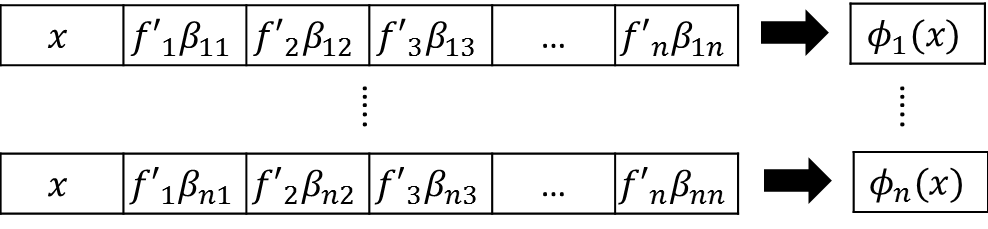
\includegraphics[scale=0.4]{fig/mktl.png}
	\caption{Illustration of feature augmentation in MKTL. $f_i'$ is the output of the $i$-th source model and $\beta_{in}$ is the hyperparameter (need to be estimated) to weigh the augmented feature. $\phi_n(x)$ is augmented feature for the $n$-th binary model.}
	\label{fig:mktl}
\end{figure}
Some previous work such as MKTL\cite{jie2011multiclass} suggests that using the prediction from the source model as the source knowledge can greatly release the constraint of the type of the source model. However, with complex feature augmentation method, there are many hyperparameters to be estimated which makes it inefficient with small training set. In this paper, we adopt the idea of using the source model prediction as the transferable knowledge and propose our transfer strategy.

Suppose we have to recognize a image from one of the $N$ visual classes and there are $N$ experts each of who can only provide the probability of this image for one certain class (binary source model). After we make our decision for one example (prediction from target model), the experts provide their own decisions as well (probabilities from the source models). Their decisions can provide extra information regarding this example as the auxiliary bias and adjust our final prediction.
As each of the experts is a specialist in one class, we should weigh their decisions as well due to the bias of their predictions (see Figure \ref{fig:ab}). 

Unlike previous work\cite{aytar2011tabula,tommasi2014learning,yang2007adapting} which has to use the specific parameter of the source model as the source knowledge, our strategy is more compatible with different types of classifiers. Compared to MKTL\cite{jie2011multiclass}, we only have to estimate $N$ hyperparameters for the $N$-class problem while there are \mbox{$N\times N$} hyperparameters in MKTL (see Figure \ref{fig:mktl}). Therefore, it is easier to estimate the transfer parameters with our strategy and EMTLe can perform better especially when the size of the training set is small.
In addition, there are two advantages of our strategy: (1) It is an effective and easy way to align the knowledge from different types of source classifiers.
(2) The auxiliary bias term is naturally normalized in the same dimension as the class probabilities are always in the interval $[0,1]$.  As EMTLe can select more types of source classifiers, this makes it more practical in a real HTL scenario.

\begin{figure}
	\centering
	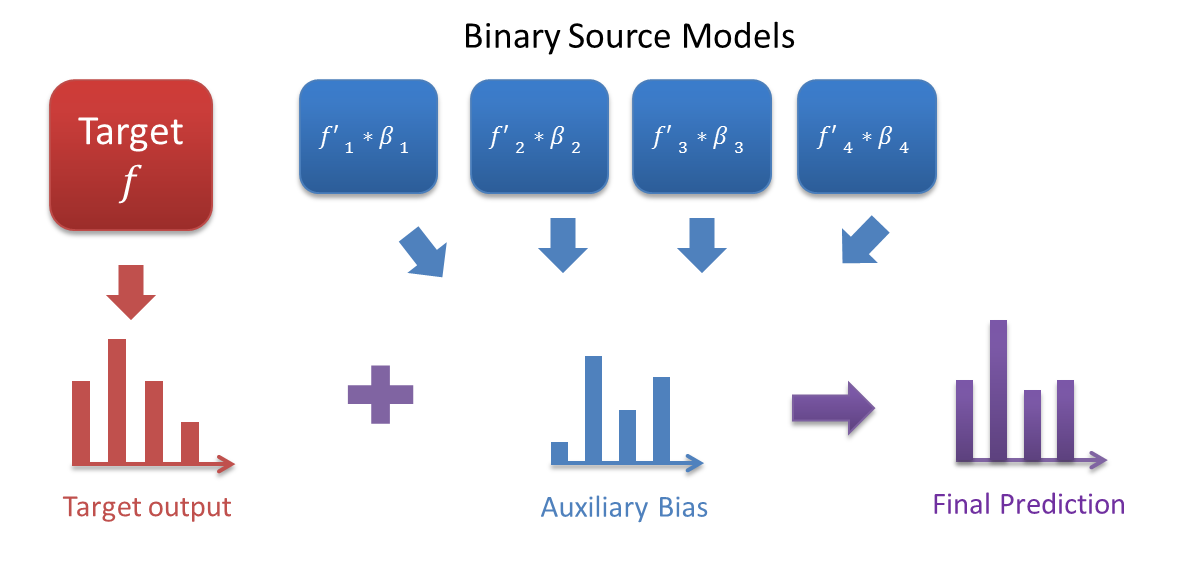
\includegraphics[scale=0.40]{fig/ab.png}
	\caption{Demonstration of using the source class probability as the auxiliary bias to adjust the output of the target model.}% $f'$ is a group of binary classifiers $\{f'_1,...,f'_4\}$ for each class and for each source model $f'_n$, we use the weight $\beta_n$ to control the knowledge transferred from this model.}
	\label{fig:ab}
\end{figure}


Here, the weight of each source model reflects the relatedness between the source model and our target domain. The more related they are, the better decision the source model can make and the larger weight we should apply to it. Specifically, in this paper, we call the weight \textit{transfer parameter}. Therefore, for any target data $D=\{x,y\}$ and the given source models $f'=\{f'_1,...,f'_N\}$, our goal is to find the target model $f$:
\begin{equation}\label{eq:low_opt}
f=\underset{f \in \mathcal{F}}{\arg \min}\ell\left(f+\beta f'|D,\beta\right)
\end{equation} 
where $\beta=[\beta_1,...,\beta_N]$ is the transfer parameter and $\ell(\cdot,\cdot)$ is the loss function to learn the target model.
It is obvious that assigning the proper transfer parameter to the source model can significantly improve the performance of our final prediction.
From Eq. \eqref{eq:low_opt} we can see that, once we have determined the value of the transfer parameter $\beta$, we are able to find the target model $f$ and solve the learning problem.
However, the transfer parameter in Eq.\eqref{eq:low_opt} is a hyperparameter and we cannot solve it directly. Therefore, we introduce our bi-level optimization method for transfer parameter estimation in the next section.







